%%
%% This is file `sample-manuscript.tex',
%% generated with the docstrip utility.
%%
%% The original source files were:
%%
%% samples.dtx  (with options: `manuscript')
%% 
%% IMPORTANT NOTICE:
%% 
%% For the copyright see the source file.
%% 
%% Any modified versions of this file must be renamed
%% with new filenames distinct from sample-manuscript.tex.
%% 
%% For distribution of the original source see the terms
%% for copying and modification in the file samples.dtx.
%% 
%% This generated file may be distributed as long as the
%% original source files, as listed above, are part of the
%% same distribution. (The sources need not necessarily be
%% in the same archive or directory.)
%%
%% The first command in your LaTeX source must be the \documentclass command.
%%%% Small single column format, used for CIE, CSUR, DTRAP, JACM, JDIQ, JEA, JERIC, JETC, PACMCGIT, TAAS, TACCESS, TACO, TALG, TALLIP (formerly TALIP), TCPS, TDSCI, TEAC, TECS, TELO, THRI, TIIS, TIOT, TISSEC, TIST, TKDD, TMIS, TOCE, TOCHI, TOCL, TOCS, TOCT, TODAES, TODS, TOIS, TOIT, TOMACS, TOMM (formerly TOMCCAP), TOMPECS, TOMS, TOPC, TOPLAS, TOPS, TOS, TOSEM, TOSN, TQC, TRETS, TSAS, TSC, TSLP, TWEB.
% \documentclass[acmsmall]{acmart}

%%%% Large single column format, used for IMWUT, JOCCH, PACMPL, POMACS, TAP, PACMHCI
% \documentclass[acmlarge,screen]{acmart}

%%%% Large double column format, used for TOG
% \documentclass[acmtog, authorversion]{acmart}

%%%% Generic manuscript mode, required for submission
%%%% and peer review
\documentclass[manuscript,screen]{acmart}

%%
%% \BibTeX command to typeset BibTeX logo in the docs
\AtBeginDocument{%
  \providecommand\BibTeX{{%
    \normalfont B\kern-0.5em{\scshape i\kern-0.25em b}\kern-0.8em\TeX}}}

%% Rights management information.  This information is sent to you
%% when you complete the rights form.  These commands have SAMPLE
%% values in them; it is your responsibility as an author to replace
%% the commands and values with those provided to you when you
%% complete the rights form.
%\setcopyright{acmcopyright}
\copyrightyear{2020}
%\acmYear{2020}
%\acmDOI{10.1145/1122445.1122456}

%% These commands are for a PROCEEDINGS abstract or paper.
%\acmConference[Woodstock '18]{Woodstock '18: ACM Symposium on Neural
 % Gaze Detection}{June 03--05, 2018}{Woodstock, NY}
%\acmBooktitle{Woodstock '18: ACM Symposium on Neural Gaze Detection,
 % June 03--05, 2018, Woodstock, NY}
%\acmPrice{15.00}
%\acmISBN{978-1-4503-XXXX-X/18/06}
\usepackage{booktabs}
\usepackage{bbding}
\usepackage{pifont}
\usepackage{wasysym}
\usepackage{amssymb}
%%
%% end of the preamble, start of the body of the document source.
\begin{document}

%%
%% The "title" command has an optional parameter,
%% allowing the author to define a "short title" to be used in page headers.
\title{A Survey of AR Piano Prototypes}

%%
%% The "author" command and its associated commands are used to define
%% the authors and their affiliations.
%% Of note is the shared affiliation of the first two authors, and the
%% "authornote" and "authornotemark" commands
%% used to denote shared contribution to the research.
\author{Jordan Aiko Deja}
%\authornote{Both authors contributed equally to this research.}
\email{jordan.deja@famnit.upr.si}
\orcid{1234-5678-9012}
\affiliation{%
  \institution{University of Primorska}
  \city{Koper}
  \country{Slovenia}
  \postcode{6000}
}

%\author{Matjaž Kljun and Klen Čopič Pucihar}
%\affiliation{%
%  \institution{Advisors}
%  \city{Koper}
 % \postcode{6000}}
%\email{\{matjaz.kljun, klen.copic\}@famnit.upr.si}

%\author{Klen Čopič Pucihar}
%\affiliation{%
%  \institution{University of Primorska}
 % \city{Koper}
  %\country{Slovenia}
  %\postcode{6000}}
%\email{klen.copic@famnit.upr.si}

%%
%% By default, the full list of authors will be used in the page
%% headers. Often, this list is too long, and will overlap
%% other information printed in the page headers. This command allows
%% the author to define a more concise list
%% of authors' names for this purpose.
\renewcommand{\shortauthors}{Deja, et al.}
%%
%% The abstract is a short summary of the work to be presented in the
%% article.
\begin{abstract}
\textbf{Abstract:} Humans have been using and learning the piano for over 3 centuries. In the last 15 years, several Augmented Reality (AR) piano prototypes that support learning have been introduced. Why are we still building these prototypes? What do these systems lack? In this paper, we present a systematic review of AR piano prototypes developed within the recent years. We review the different innovations they present and organise them into contribution categories. We will then discuss the impact of these contributions and recommend directions for future work towards designing better AR piano prototypes and conducting user studies.
\end{abstract}
%%
%% The code below is generated by the tool at http://dl.acm.org/ccs.cfm.
%% Please copy and paste the code instead of the example below.
%%
\begin{CCSXML}
<ccs2012>
   <concept>
       <concept_id>10003120.10003138.10011767</concept_id>
       <concept_desc>Human-centered computing~Empirical studies in ubiquitous and mobile computing</concept_desc>
       <concept_significance>500</concept_significance>
       </concept>
 </ccs2012>
\end{CCSXML}
\ccsdesc[500]{Human-centered computing~Empirical studies in ubiquitous and mobile computing}
%%
%% Keywords. The author(s) should pick words that accurately describe
%% the work being presented. Separate the keywords with commas.
\keywords{augmented reality, piano, meta-analysis, prototypes}
%%
%% This command processes the author and affiliation and title
%% information and builds the first part of the formatted document.
\maketitle

\section{Introduction}
In around the year 1700, the piano, an elegant yet complex to use musical instrument was invented. Since then, humans have been designing innovations improving the experiences of learning and playing the piano. Several technology interventions have been introduced to assist in these scenarios. As these contributions are presented, changes in the way humans use the piano and technology also take place. This is because of the affordances affecting users that go with these technologies. One of these innovations is through Augmented Reality (AR). The earliest known prototype designed with AR came in the late 90s in the form of a musical keyboard display with keyboard input method \cite{breitweiser1996musical}. This along with other AR prototypes rode the waves of the Information era, with the boom of the World Wide Web, the emergence of the millennium bug, higher resolution graphics, stronger processors and better tracking algorithms among many others. Since then, as several AR piano prototypes have been developed, key innovations have shifted focus as well jumping from one technology to other (e.g. overlaying graphics to optimization to teaching modes). As these innovations shift focus from one to the other, human experiences are also reshaped by these changes. 

\citet{dede1996evolution} contends that technological media (such as computers) provide affordances that play an important role in the use and teaching with technology. 


\subsection{Objectives}

Survey of AR piano teaching systems and prototypes
Discussion on how these prototypes were evaluated and how the research focus has changed over the last 15 years
Overview of what technological contributions were made and future steps 

.. This paper focuses on X prototypes categorized and sorted by .. These sections describe prototypes that addressed problems in (enumerate). In each section, prototypes are grouped in subsection compared by its .. They are also listed in chronological order to show the course of development. Each subsection ends with a short discussion about .. This paper concludes with an overview discussion and a conclusion about ..

\subsection{Organization}
The paper is organized as follows: Section 2 discusses our definition of Augmented Reality (AR) piano prototypes and a background on the piano learning process. Section 3 describes our methods for qualitative analysis. Section 4 discusses the results of our analysis of the trends in AR piano prototypes designed throughout the years. Section 5 discusses the results of our qualitative analysis of AR piano prototypes covering state-of-the-art contributions (in the design, engineering and content). We organise these strategies into categories such as hand tracking, visualisations, agents and tutors, and learning modes in Section 5. We also look at the evaluation aspect of these studies and the analyses that go with them as covered in Section 6. Lastly, Section 7 concludes this paper with our recommendation for future AR piano prototypes. 





\section{Background}
\subsection{Piano Learning}
How do people learn the piano? what are the different stages of learning the piano? what stages in piano learning have been augmented by technology? what are the existing gaps in this process? How much virtuality (in miligram's continuum) has been included in piano? 

\subsection{Augmented Reality Piano Prototypes}
Augmented Reality
Augmented reality piano teaching systems
Design Factors affecting augmented reality piano teaching systems (hardware, software, content)

\section{Method}

We did a literature review following the \textbf{Preferred Reporting Items for Systematic Reviews and Meta-Analyses} technique, also known as PRISMA \cite{moher2009preferred}. The work of \citet{santos2013augmented} which has reviewed AR learning environments has applied PRISMA techniques as well. This guided us further on how to analyse and review AR prototypes for this specific context. The approach included a  qualitative-analysis phase that aims to review these innovations in a specific context. The methodology for this systematic review is as follows: 

\subsection{Search for Prototypes}
\label{subsec: search}
We did a literature search between March to August 2020 in several digital libraries such as Google Scholar, ACM Digital Library and IEEE Xplore Digital Library. The search strings used where:
\begin{enumerate}
    \item "augmented reality piano"
    \item "AR piano"
    \item "augmented reality keyboard"
    \item "AR keyboard"
\end{enumerate}
The search included journal articles, conference proceedings and patents that are written in English. Some articles were not written in English but had available translations. A total of 316 articles were found from this initial search from these online libraries. 
\subsection{Inclusion Criteria}
\label{subsec: criteria}
The focus of this survey is on AR piano prototypes. We needed to further filter these articles based on the following criteria:
\begin{enumerate}
    \item The research paper discusses an AR piano prototype 
    \item The AR piano prototype is meant for playing, learning or teaching the piano
    \item The prototype has a component that makes it qualified as augmented reality
    %\item The full research paper is publicly accessible 
\end{enumerate}
These inclusion criteria were manually done at the best judgment of the author. Following this criteria, we resulted to forty (40) articles. Moreover, not all these prototypes immediately qualify based on the definition of AR. Prototypes that make use of both 2D and 3D are considered. Prototypes that simulate the effect of AR even if they do not implement the tracking of an object were also included in this review. 

\subsection{Qualitative Analysis}
We performed a qualitative analysis of the different papers retried after performing the steps at subsection \ref{subsec: search}. We used the criteria defined in subsection \ref{subsec: criteria}. This gave us a clearer understanding of the prototypes in these articles. Note that these 40 articles do not represent 40 unique prototypes because a small fraction of these studies discussed advancements in the development of the same prototype. \\

\subsection{Data Gathering}
A form was drafted to facilitate the gathering of data from the 40 included articles. The form seeks to retrieve the following information: 
\begin{enumerate}
    \item publication details
    \item contributions
    \item use of AR
    \item citation count
    \item design and results of the user study
\end{enumerate}
The publication details include the title of the paper, year of publication, authors etc. The contributions of each paper were extracted and analyzed as well. The use of AR refers to the set of features that describe its AR component. This can refer to as head-mounted, agent-based, mobile, etc. The design and results of the user study refer to the description of applicable user studies and tests. Other features include sample size, method, questionnaire and tools used to conduct the user tests. \\

The review was designed to easily recognize common trends among the papers included in this study. Data and findings were sorted towards supporting any form of further data gathering. Note that the goal is not to correctly describe which prototype is an AR piano or not but to gather enough examples of prototypes that have effectively used AR as a technique in playing or learning the piano.  
\section{Trends in AR Piano Prototypes}

sample thought: when did hand tracking get popular and how spread out are they throughout the years 

\begin{table}[]
\caption{Table of studies and a checklist of their features based on contribution categories as described in section \ref{tab: all}. Legend: \textbf{\#}= number of citations; \textbf{KB}= AR keyboard; \textbf{AT}= AR agents and tutors; \textbf{PR}= piano roll and other visuals that simplify chords and notes; \textbf{US}= user study; \textbf{HT}= hand tracking; \textbf{LM}= learning modes.}
\small\begin{tabular}{llrrccccccl}
\hline \hline
\textbf{Paper} & \textbf{Author} & \textbf{Year} & \textbf{\#} & \textbf{KB} & \textbf{AT} & \textbf{PR} & \textbf{US} & \textbf{HT} & \textbf{LM} & \textbf{Others} \\ \hline
P1    & \citet{huang2011piano}              & 2011 & 50         & \ding{51} &           &           &           & \ding{51} &           & \\ \hline
P2    & \citet{nugraha2014pemanfaatan}      & 2014 & 38         & \ding{51} &           &           & \ding{51} &           &           & \\ \hline
P3    & \citet{barakonyi2005augmented}      & 2005 & 47         & \ding{51} & \ding{51} & \ding{51} &           &           & \ding{51} & \\ \hline
P4    & \citet{chow2013music}               & 2013 & 45         & \ding{51} &           & \ding{51} & \ding{51} &           & \ding{51} & \\ \hline
P5    & \citet{weing2013piano}              & 2013 & 29         &           &           & \ding{51} & \ding{51} & \ding{51} & \ding{51} & \textit{gamified viz}\\ \hline
P6    & \citet{hackl2017holokeys}           & 2017 & 7          & \ding{51} &           & \ding{51} &           &           &           & \\ \hline
P7    & \citet{chouvatut2013virtual}        & 2013 & 8          & \ding{51} &           & \ding{51} &           &           &           & \textit{supports PWD's}\\ \hline
P8    & \citet{fernandez2016piano}          & 2016 & 7          &           & \ding{51} & \ding{51} &           &           &           & \\ \hline
P9    & \citet{das2017music}                & 2017 & 5          & \ding{51} & \ding{51} & \ding{51} &           &           & \ding{51} & \textit{lesson builder} \\ \hline
P10   &  \citet{claudia2017yousician}       & 2017 & 0          &           &           & \ding{51} &           &           &           & \\ \hline
P11   & \citet{trujano2018arpiano}          & 2018 & 4          & \ding{51} &           & \ding{51} &           &           &           & \\ \hline
P12   & \citet{kerdvibulvech2017innovative} & 2017 & 4          & \ding{51} &           &           & \ding{51} & \ding{51} &           & \textit{users gesture on air}\\ \hline
P13   & \citet{oka2013marker}               & 2013 & 27         &           &           &           &           & \ding{51} &           & \textit{piano fingering}\\ \hline
P14   &  \citet{liang2016barehanded}        & 2016 & 20         & \ding{51} &           &           &           & \ding{51} &           & \\ \hline
P15   & \citet{schmalstieg2007experiences}  & 2007 & 268        &           &           & \ding{51} & \ding{51} &           &           & \\ \hline
P16   & \citet{correa2009computer}          & 2009 & 63         & \ding{51} &           & \ding{51} & \ding{51} &           &           & \textit{patients w/ cerebral palsy}\\ \hline
P17   & \citet{xiao2014andante}             & 2014 & 28         &           & \ding{51} & \ding{51} &           &           & \ding{51} & \\ \hline 
P18   & \citet{takegawa2012piano}           & 2012 & 26         &           &           & \ding{51} & \ding{51} &           & \ding{51} & \\ \hline 
P19   & \citet{xiao2010mirrorfugue}         & 2011 & 31         &           & \ding{51} & \ding{51} & \ding{51} &           &           & \textit{3 unique interfaces}\\ \hline
P20   & \citet{xiao2013mirrorfugue}         & 2013 & 17         &           & \ding{51} &           & \ding{51} &           &           & \\ \hline
P21   & \citet{li2018application}           & 2018 & 1          & \ding{51} &           &           & \ding{51} &           &           & \\ \hline 
%P22   & \citet{wei2015teaching}             & 2015 & 154        &                  &       &        &    &  & &             \\
P22   & \citet{zaqout2015augmented}         & 2015 & 1          & \ding{51} &           &           &           &           &           & \\ \hline 
%P24   & \citet{serafin2017considerations}   & 2017 & 25         &                  &       &         &   &  & &             \\
P23   & \citet{leonard2013virtual}          & 2013 & 9          & \ding{51} &           &           & \ding{51} &           &           & \\ \hline 
P24   & \citet{raymaekers2014game}          & 2014 & 14         &           &           & \ding{51} & \ding{51} &           & \ding{51} & \textit{shooting game}\\ \hline
P25   & \citet{rogers2014piano}             & 2017 & 42         &           &           & \ding{51} & \ding{51} &           & \ding{51} & \\ \hline
P26   & \citet{birhanu2017keynvision}       & 2017 & 2          &           &           & \ding{51} &           &           & \ding{51} & \\ \hline
P27   & \citet{sun2018mr}                   & 2018 & 3          & \ding{51} &           & \ding{51} & \ding{51} &           &           & \textit{one and two hand modes}\\ \hline
P28   & \citet{goodwin2013key}              & 2013 & 10         &           & \ding{51} & \ding{51} &           &           &           & \\ \hline
P29   & \citet{zeng2019funpianoar}          & 2019 & 2          &           &           &           &           &           &           & \textit{used ar markers}\\ \hline
P30   & \citet{de2014infrared}              & 2014 & 6          & \ding{51} &           &           &           & \ding{51} &           & \textit{magnetic glove}\\ \hline
P31   & \citet{molloy2019mixed}             & 2019 & 1          &           &           & \ding{51} & \ding{51} &           & \ding{51} & \textit{cognitive load, motivation}\\ \hline
%P34   &  \citet{zaqout2015augmented}        & 2015 & 1          &                  &       &          &  &      & &         \\
P32   & \citet{cai2019designa}               & 2019 & 1         &           &           & \ding{51} &           &           & \ding{51} & \textit{formal \& competition mode}\\ \hline
P33   & \citet{gerry2019adept}              & 2019 & 2          &           & \ding{51} & \ding{51} &           & \ding{51} &           & \textit{leap motion capture}\\ \hline 
P34   & \citet{zhang2010affordable}         & 2010 & 22         & \ding{51} &           &           &           &           &           & \\ \hline 
P35   &  \citet{pan2018pilot}               & 2018 & 2          & \ding{51} &           &           & \ding{51} &           &           & \textit{single \& pair modes}\\ \hline
P36   &  \citet{cai2019designb}              & 2019 & 0         &           &           & \ding{51} &           & \ding{51} &           & \textit{group piano}\\ \hline
%P40   &  \citet{poupyrev2001augmented}      & 2001 & 27         &                  &       &         &   &     & &          \\
P37   & \citet{sandnes2019enhanced}         & 2019 & 0          &           &           & \ding{51} &           &           &           & \\ \hline
P38   & \citet{kim2014ar}                   & 2014 & 11         & \ding{51} &           & \ding{51} & \ding{51} &           &           & \\ \hline
%P43   & \citet{zeng2019new}                 & 2019 & 0          &                  &       &        &    &    & &           \\
P39   &  \citet{xiao2011duet}               & 2011 & 7          &           &           & \ding{51} & \ding{51} &           & \ding{51} & \textit{practice modes}\\ \hline 
P40   & \citet{xu20195}                     & 2019 & 0          &           & \ding{51} & \ding{51} &           &           & \ding{51} & \textit{self reflection}\\ \hline 
%P46   & \citet{oku2019novel}                & 2019 & 2          &                  &       &         &   &     & &          \\
%P47   & \citet{birhanu2017interactive}      & 2017 & 0          &                  &       &         &   &      & &         \\
%P48   &  \citet{rahman2013hand}             & 2013 & 6          &                  &       &         &   &     & &          \\
%P49   & \citet{mostafizur2011application}   & 2011 & 5          &                  &       &         &   &       & &        \\ \hline
      &                                     &           & \textit{\={x}}=21 & 47\% & 22\% & 67\%    & 45\%      & 20\%      & 32\%      & \\ \hline \hline
\label{tab:overview}
\end{tabular}
\end{table}

\begin{figure}
    \centering
    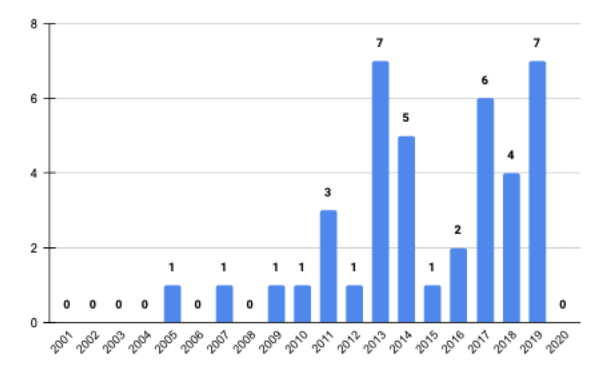
\includegraphics[width=10cm]{figures/articlexyear.png}
    \caption{ Number of AR piano prototype papers published within the last 2 decades }
    \label{fig:articleyeartrend}
\end{figure}

\begin{figure}
    \centering
    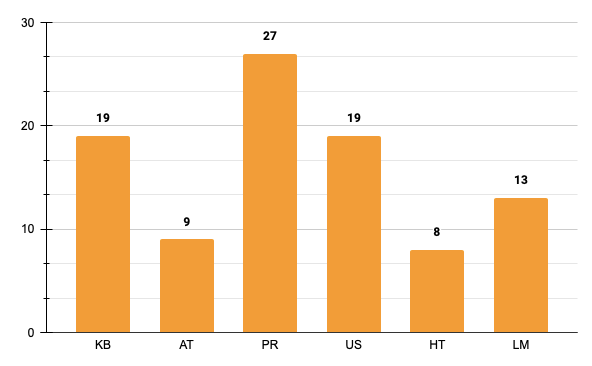
\includegraphics[width=10cm]{figures/typecount.png}
    \caption{Comparison of AR piano prototype contribution categories}
    \label{fig:typecount}
\end{figure}

\begin{figure}
    \centering
    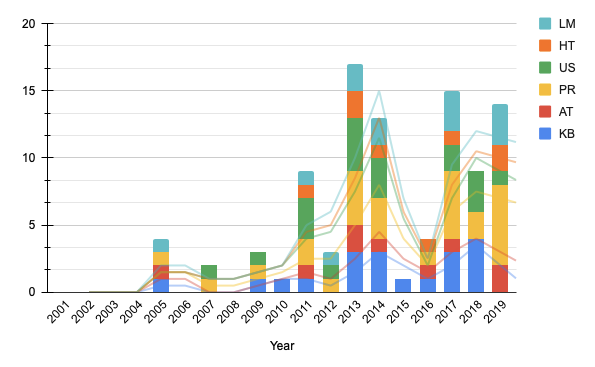
\includegraphics[width=15cm]{figures/typeyeartrend.png}
    \caption{Trend of AR piano prototype contribution categories within the last 2 decades}
    \label{fig:typeyeartrend}
\end{figure}


\section{Strategies in Designing AR Pianos}
\label{sec: strat}
\subsection{Hand Tracking}
something here 
\subsection{Visualisations}
Section discussing prototypes whose main contributions focused on visualizations, overlaying graphics, rendering and optimization etc
\subsection{Agents and Tutors}
Section discussing prototype whose main contributions focused on virtual agents/tutors 
\subsection{Learning Modes}
Section discussing prototype whose contributions focused on learning modes, emphasis on pedagogy and other learner-centric modes
\section{Evaluation Techniques}
done by studies on AR piano teaching systems (hypothesis based on cognition, realistic annotations etc)

% Please add the following required packages to your document preamble:
% \usepackage{graphicx}
\begin{table}[]
\caption{Table of Studies from \ref{tab:overview} with user studies. This table provides an overview of their techniques, treatments and tools used.}
\label{tab: us-all}
\resizebox{\textwidth}{!}{%
\begin{tabular}{lllllll} \hline \hline
\textbf{Ref.}                           & \textit{n}    & \textbf{treatment}    & \textbf{metrics constructs}    & \textbf{tools}\\ \hline
%P1 \cite{huang2011piano}              & 2011 &        & a                         & a                             & a                    \\
\cite{nugraha2014pemanfaatan}        & 8                & major and minor chords animated marker detection & usability, operation, attraction & self made questionnaire \\
\cite{chow2013music}                 & 7                & play a piece in the piano & usage, benefit, system rating & open ended questions \\
\cite{weing2013piano}                & 5                & practice and exploration modes & finger information, notation, satisfaction, cognitive load & self made questionnaire \\
\cite{kerdvibulvech2017innovative}  & 1                 & play a piece in the piano & scoring, time interval        & time tracking        \\
\cite{schmalstieg2007experiences}   & 0                 & a                         & a                             & a                    \\
\cite{correa2009computer}           & 0                 & a                         & a                             & a                    \\
\cite{takegawa2012piano}            & 0                 & a                         & a                             & a                    \\
\cite{xiao2010mirrorfugue}          & 0                 & a                         & a                             & a                    \\
\cite{xiao2013mirrorfugue}          & 0                 & a                         & a                             & a                    \\
\cite{li2018application}            & 0                 & a                         & a                             & a                    \\
\cite{leonard2013virtual}           & 0                 & a                         & a                             & a                    \\
\cite{raymaekers2014game}           & 0                 & a                         & a                             & a                    \\
\cite{rogers2014piano}              & 0                 & a                         & a                             & a                    \\
\cite{sun2018mr}                    & 0                 & a                         & a                             & a                    \\
\cite{molloy2019mixed}              & 0                 & a                         & a                             & a                    \\
\cite{pan2018pilot}                 & 0                 & a                         & a                             & a                    \\
\cite{kim2014ar}                    & 0                 & a                         & a                             & a                    \\
\cite{xiao2011duet}                 & 0                 & x                         & x                             & x                   \\ \hline 
                                    & \textit{\={x}}=6      &                      &                               &                   \\ \hline \hline 
\end{tabular}%
}
\end{table}




\section{Discussion and Future Directions}

gaps in modelling? position near your thesis

\section{Tables and Figures}
Figure of number of participants per study by years, size of each bubble is relative to sizes of other bubbles and based on number of participants in a study. Sort per category 

Figure/Table of all described prototypes with year, by type with number of participants, short study description, number of citations

Table of Studies evaluating learner performance with effect sizes (content, sample, control group, treatment, effect, size)

Table of Studies evaluating learner performance 

Figure of number of AR piano teaching system publications until june 2020

Table of AR piano teaching systems with corresponding devices 

Table of AR piano teaching systems showing summary of survey
questionnaires

%\begin{figure}
%    \centering
%    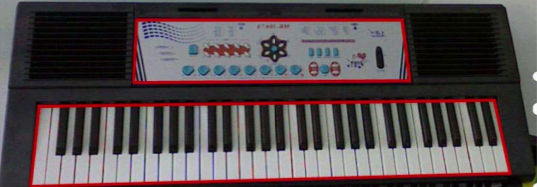
\includegraphics[width=7cm]{figures/pianomarker.png}
 %   \caption{Piano Augmented Reality marker}
 %   \label{fig:pianomarker}
%\end{figure}

%\begin{figure}
%    \centering
%    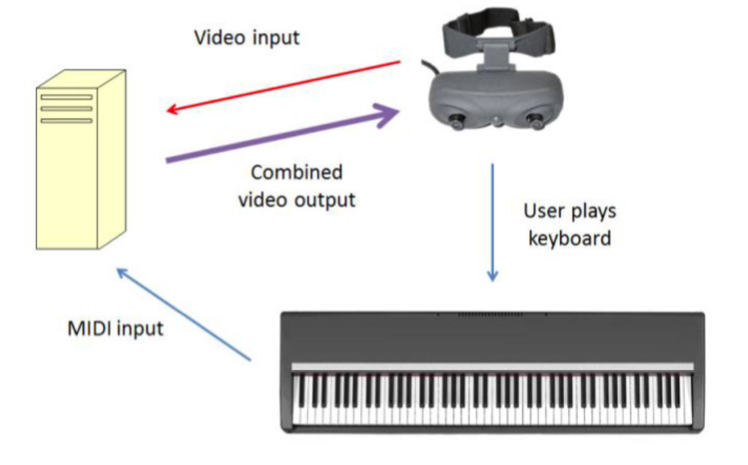
\includegraphics[width=7cm]{figures/headmountedpiano1.png}
 %   \caption{Architecture of the Head Mounted Piano by cite! }
%    \label{fig:pianoheadmountedarch}
%\end{figure}

%\begin{figure}
%    \centering
 %   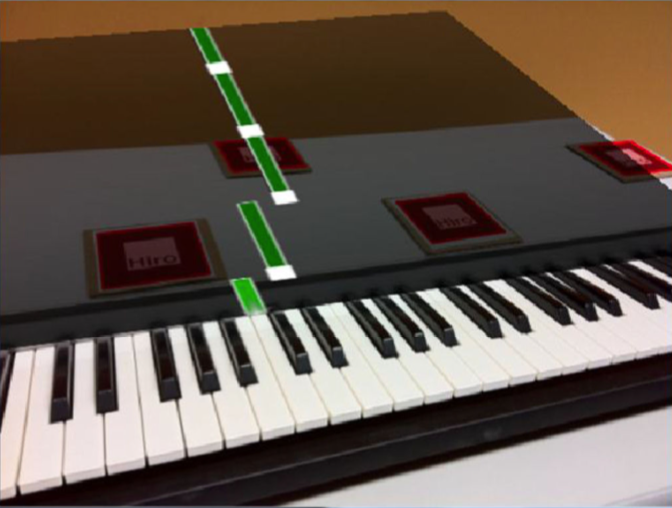
\includegraphics[width=7cm]{figures/headmountedview.png}
 %   \caption{View from the Head Mounted Piano AR  }
 %   \label{fig:View from the HeadMounted}
%\end{figure}

\begin{figure}
    \centering
    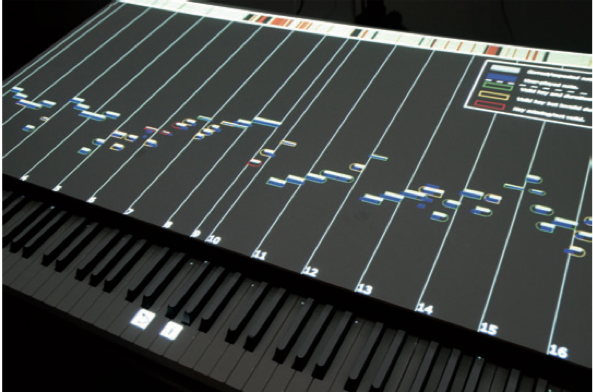
\includegraphics[width=7cm]{figures/piano}
    \caption{\cite{rogers2014piano}}
    \label{fig:rogers2014piano}
\end{figure}

\begin{figure}
    \centering
    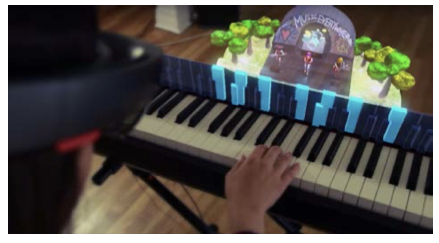
\includegraphics[width=7cm]{figures/daspiano.png}
    \caption{\cite{das2017music} }
    \label{fig:daspiano}
\end{figure}

\begin{figure}
    \centering
    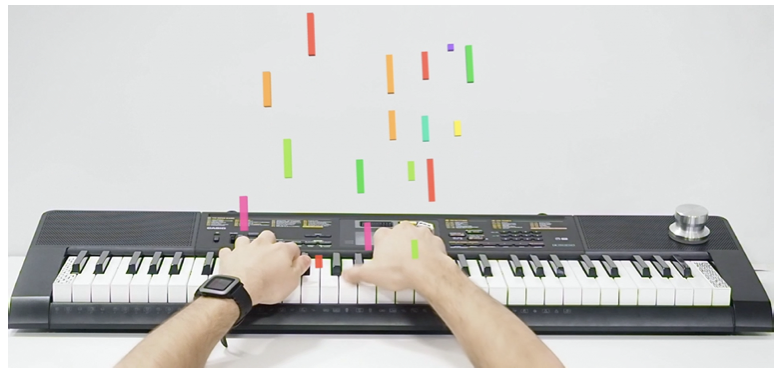
\includegraphics[width=15cm]{figures/arpianotrujano.png}
    \caption{\cite{trujano2018arpiano} }
    \label{fig:View from the HeadMounted}
\end{figure}

\begin{figure}
    \centering
    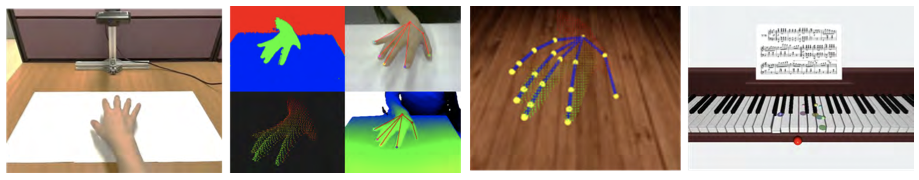
\includegraphics[width=15cm]{figures/lianghandtrack.png}
    \caption{\cite{liang2016barehanded} }
    \label{fig:View from the HeadMounted}
\end{figure}

\begin{figure}
    \centering
    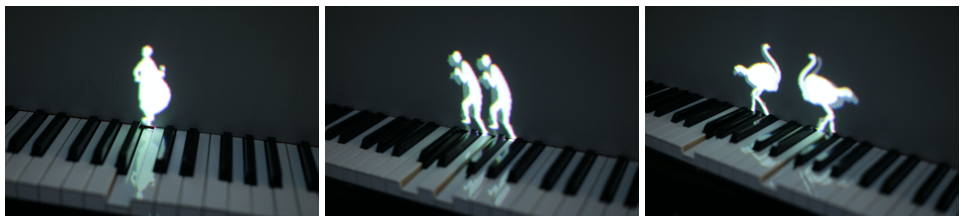
\includegraphics[width=15cm]{figures/xiaoandante.png}
    \caption{\cite{xiao2014andante} }
    \label{fig:View from the HeadMounted}
\end{figure}

\begin{figure}
    \centering
    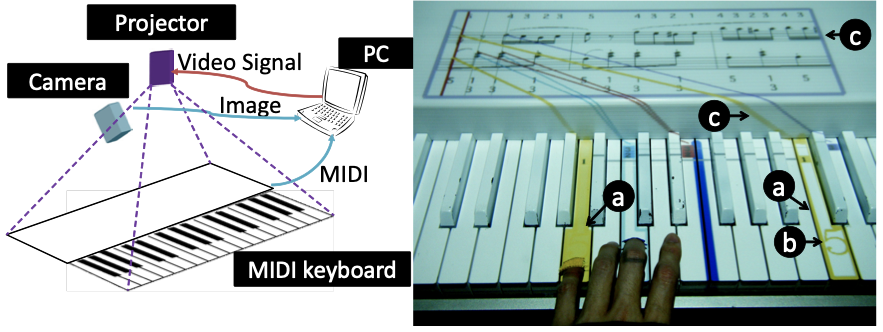
\includegraphics[width=15cm]{figures/takegawasetup.png}
    \caption{\cite{takegawa2012piano} }
    \label{fig:View from the HeadMounted}
\end{figure}

\begin{figure}
    \centering
    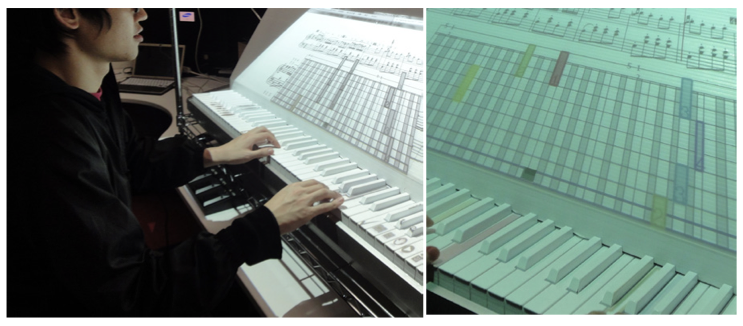
\includegraphics[width=15cm]{figures/takegawapianoroll.png}
    \caption{\cite{takegawa2012piano} }
    \label{fig:View from the HeadMounted}
\end{figure}

\begin{figure}
    \centering
    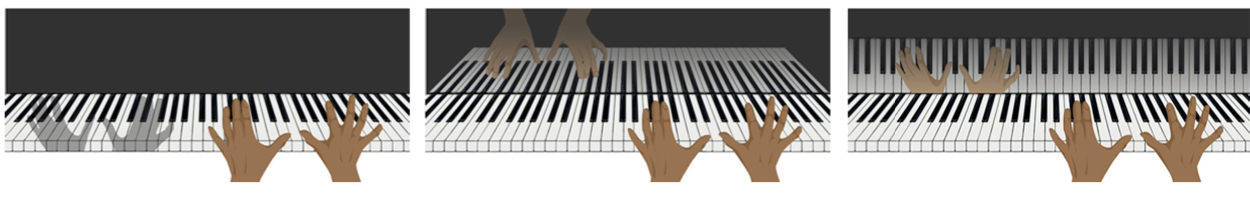
\includegraphics[width=15cm]{figures/xiaomirror3interfaces.png}
    \caption{\cite{xiao2010mirrorfugue} }
    \label{fig:View from the HeadMounted}
\end{figure}

\begin{figure}
    \centering
    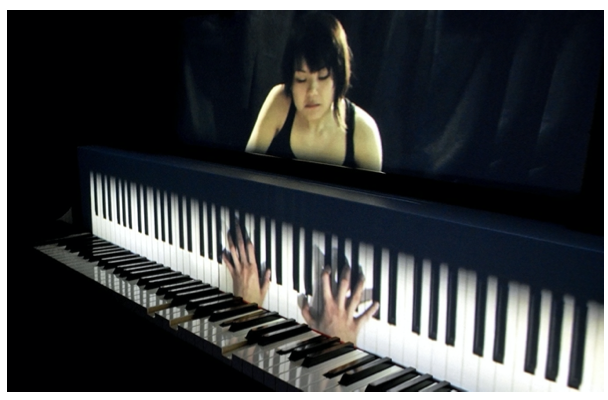
\includegraphics[width=7cm]{figures/xiaomirrorfugue3.png}
    \caption{\cite{xiao2013mirrorfugue} }
    \label{fig:xiao2013mirror}
\end{figure}

\begin{figure}
    \centering
    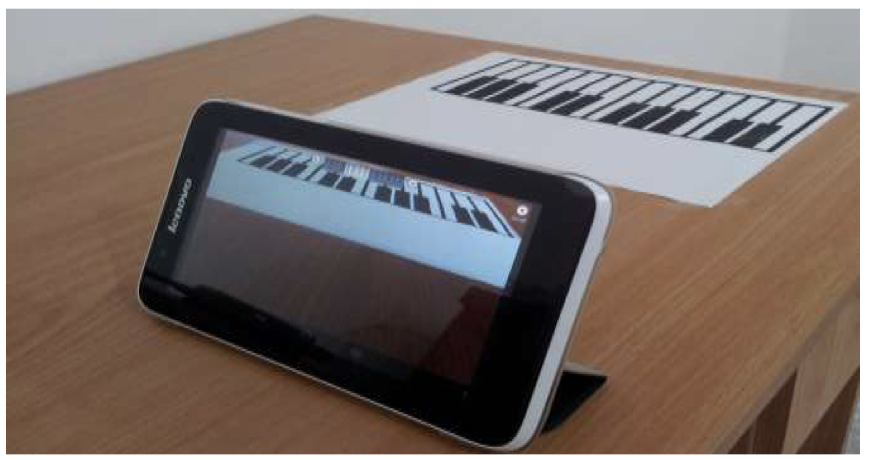
\includegraphics[width=7cm]{figures/zaqoutfingerpiano.png}
    \caption{\cite{zaqout2015augmented} }
    \label{fig:zaqoutfingerpiano}
\end{figure}

\begin{figure}
    \centering
    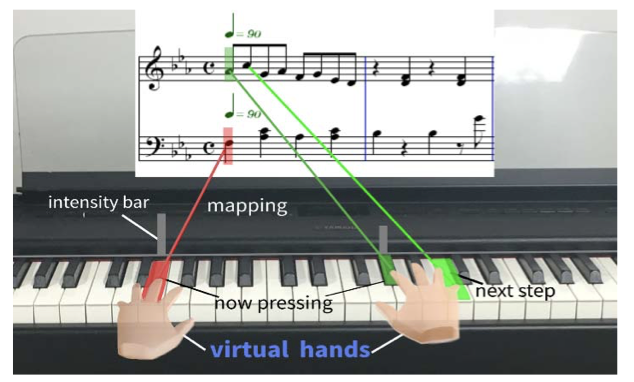
\includegraphics[width=7cm]{figures/caipiano.png}
    \caption{\cite{cai2019designa} }
    \label{fig:caipiano}
\end{figure}


\begin{figure}
    \centering
    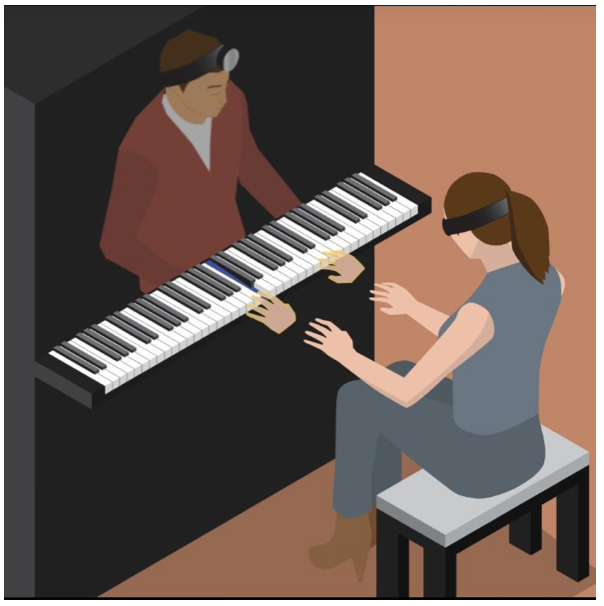
\includegraphics[width=7cm]{figures/gerryadept.png}
    \caption{\cite{gerry2019adept} }
    \label{fig:gerryadept}
\end{figure}

\begin{figure}
    \centering
    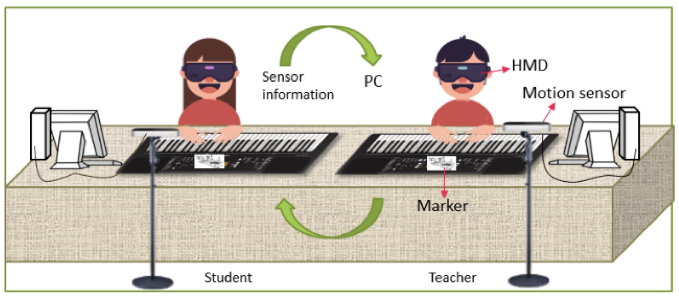
\includegraphics[width=7cm]{figures/caigroup.png}
    \caption{\cite{cai2019designb} }
    \label{fig:caigroup}
\end{figure}

\begin{figure}
    \centering
    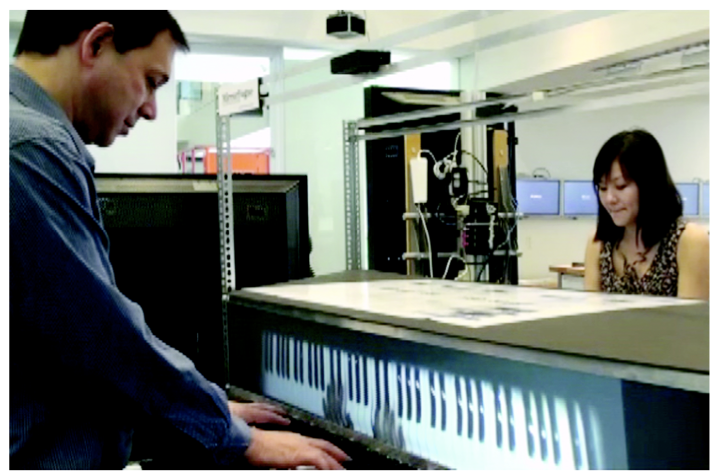
\includegraphics[width=7cm]{figures/xiaomrror2011.png}
    \caption{\cite{xiao2011duet} }
    \label{fig:xiaomirror2011}
\end{figure}

%%
%% The next two lines define the bibliography style to be used, and
%% the bibliography file.
\bibliographystyle{ACM-Reference-Format}
\bibliography{sample-base}
%%
%\nocite{*}
%% If your work has an appendix, this is the place to put it.
%\appendix
\end{document}
\endinput
%%
%% End of file `sample-manuscript.tex'.
